\documentclass[12pt,a4paper]{ctexart}
\usepackage{geometry}
\geometry{left=2.5cm,right=2.5cm,top=2.5cm,bottom=2.5cm}
\usepackage{listings}
\usepackage{xcolor}
\usepackage{booktabs}
\usepackage{amsmath}
\usepackage{tikz}
\usetikzlibrary{arrows}
\usepackage{graphicx}
\usepackage{tcolorbox}
\tcbuselibrary{skins,breakable}
\usepackage[colorlinks,linkcolor=blue!70!black,urlcolor=blue!60!black]{hyperref}

\definecolor{themecolor}{RGB}{30,64,175}
\definecolor{codebg}{RGB}{245,247,250}
\definecolor{codeframe}{RGB}{100,116,139}

\usepackage{titlesec}
\titleformat{\section}{\Large\bfseries\color{themecolor}}{\thesection}{0.8em}{}[\vspace{-0.5em}\rule{\textwidth}{0.4pt}]
\titlespacing*{\section}{0pt}{1.2em}{0.6em}
\titleformat{\subsection}{\large\bfseries\color{themecolor!80}}{\thesubsection}{0.8em}{}
\titlespacing*{\subsection}{0pt}{0.8em}{0.3em}

\lstset{
  basicstyle=\small\ttfamily,
  keywordstyle=\color{blue!80!black}\bfseries,
  commentstyle=\color{green!50!black}\itshape,
  stringstyle=\color{red!70!black},
  numbers=left,numberstyle=\tiny\color{gray},
  backgroundcolor=\color{codebg},
  frame=single,rulecolor=\color{codeframe!40},
  breaklines=true,breakatwhitespace=true,
  language=C++,
  aboveskip=0.8em,belowskip=0.6em
}

\newtcolorbox{webox}{colback=blue!5!white,colframe=themecolor,coltitle=white,fonttitle=\bfseries,title=Web前端展示,boxrule=0.5pt,arc=3pt}

\title{\textbf{编译器设计专题实验报告}\\[0.5em]\Large\color{themecolor}实验三：LR(0)项目集规范族生成}
\author{张凌曜 \quad 2234214014 \quad 计算机2306}
\date{}

\begin{document}
\maketitle

\section{实验目的}
构建给定文法的LR(0)项目集规范族，计算每个状态的闭包和Goto转移，并判断文法是不是LR(0)文法。

\section{实验原理}
LR(0)项目就是在产生式右部放个圆点``$\cdot$''表示分析到哪了。比如$E \to \cdot E + T$表示正在识别$E+T$但还没读入东西。

闭包运算：如果项目集里有点在非终结符前面的项目（$A \to \alpha \cdot B \beta$），就把$B$的所有产生式加上点在开头加进去，反复做直到没有新的了。

Goto运算：把项目集里点前有$X$的项目的点往右移一位，然后对结果再求闭包。

冲突判断：某个状态里同时有移进项目和归约项目就是移进-归约冲突，多个归约项目就是归约-归约冲突。有冲突就不是LR(0)文法。

\section{实验过程}

\subsection{文法输入}
程序读取产生式，用\texttt{->}表示推导，\texttt{|}分隔多个右部：

\begin{lstlisting}[language={}]
# 四则运算表达式文法
E -> E + T | T
T -> T * F | F
F -> ( E ) | id
\end{lstlisting}

程序自动加增广产生式$E' \to E$。

\subsection{实现要点}
闭包用工作队列实现，避免重复处理。项目集用\texttt{set}存，天然去重。规范族的构建用BFS，对每个状态尝试所有符号的Goto，如果得到的项目集已存在就记录转移，否则加为新状态。

\section{测试结果}

\subsection{四则运算文法}
$E \to E + T | T$，$T \to T * F | F$，$F \to (E) | id$

程序输出12个状态、22个转移函数。部分状态：

\begin{table}[h]
\centering
\begin{tabular}{l}
\toprule
$I_0$: $E' \to \cdot E$, $E \to \cdot E+T$, $E \to \cdot T$, $T \to \cdot T*F$, $T \to \cdot F$, $F \to \cdot(E)$, $F \to \cdot id$ \\
$I_1$: $E \to \cdot E+T$, $F \to (\cdot E)$, $E \to \cdot T$, $T \to \cdot T*F$, $T \to \cdot F$, $F \to \cdot(E)$, $F \to \cdot id$ \\
$I_2$: $E' \to E\cdot$, $E \to E\cdot +T$ \\
\bottomrule
\end{tabular}
\end{table}

$I_2$里$E' \to E\cdot$是归约，$E \to E\cdot+T$是移进，存在移进-归约冲突。$I_4$和$I_{10}$也有类似问题。所以\textbf{这个文法不是LR(0)的}。

\begin{center}
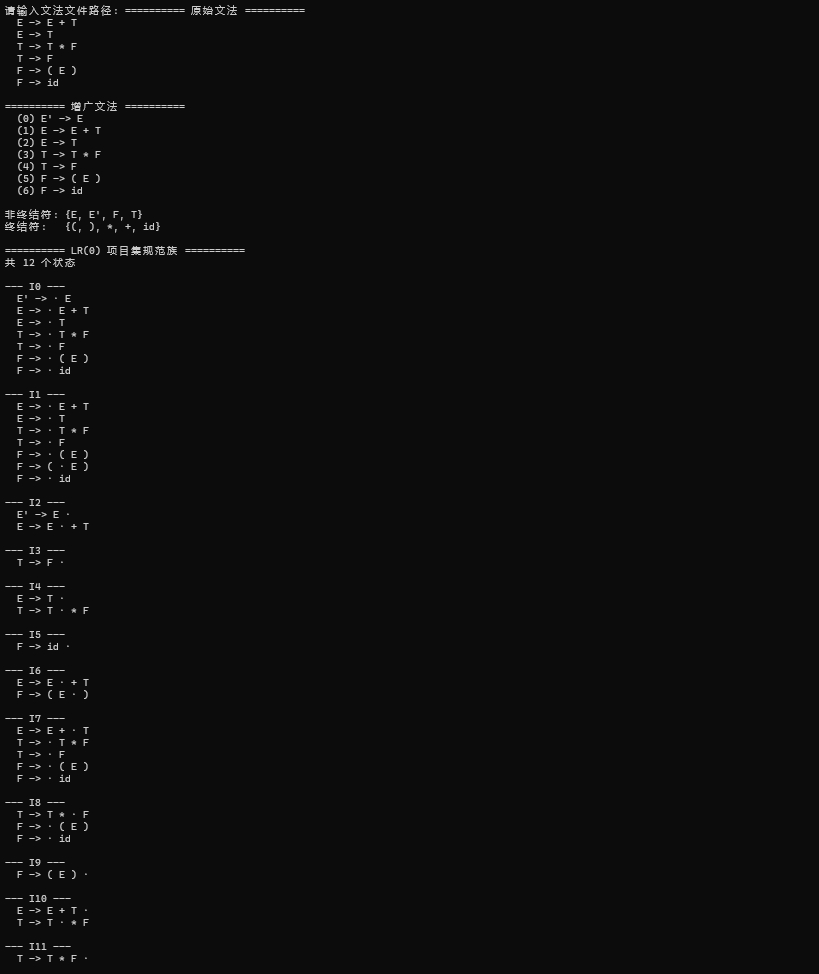
\includegraphics[width=0.9\textwidth]{image/1.1.png}
\vspace{0.5em}
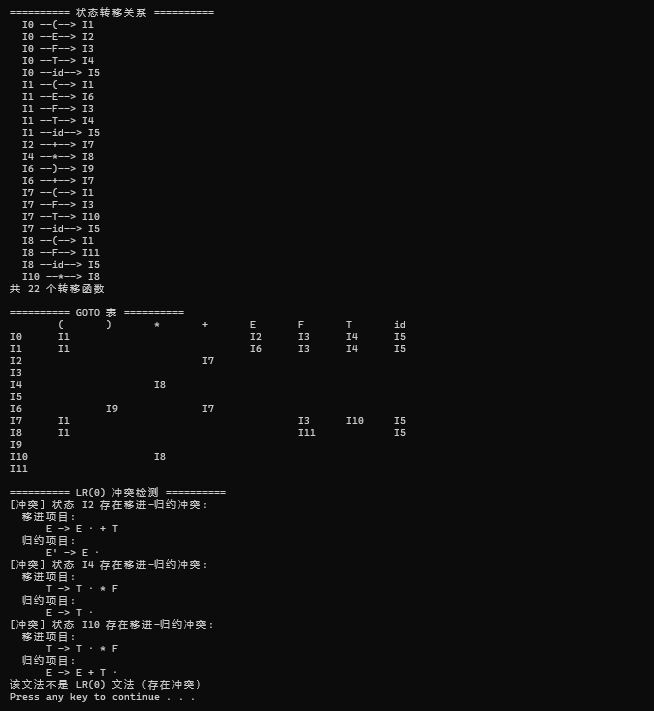
\includegraphics[width=0.9\textwidth]{image/1.2.png}
\end{center}

\subsection{简单文法}
$S \to aB$, $B \to bB | c$

生成6个状态、7个转移，没有冲突，\textbf{是LR(0)文法}。

\begin{center}
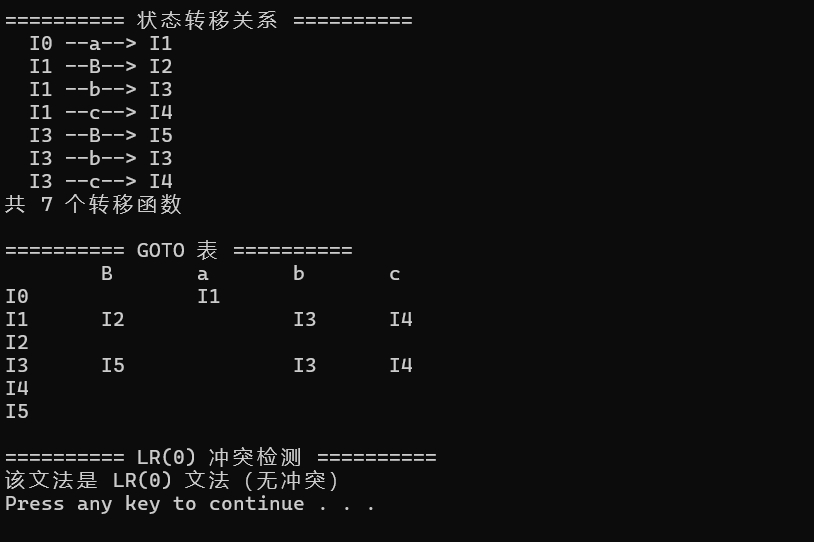
\includegraphics[width=0.9\textwidth]{image/2.1.png}
\end{center}

\section{问答题：DFA词法规则与报错分析}
用第一个DFA作为词法规则扫描\texttt{test.src}（内容为\texttt{x = 42 + y}）时，程序报了大量错误。

原因：第一个DFA的转移函数设计得比较简单，只能识别很少的Token类型。遇到不在其字符集范围内的字符就会拒绝：字母\texttt{x}、\texttt{y}没有定义识别转移，所以报\texttt{Invalid character}；赋值符\texttt{=}也不在DFA的转移表中；部分数字和运算符同样超出DFA的处理范围。最后一个\texttt{Invalid DFA state 3}说明DFA在识别某个运算符时进入了一个没有出边的死状态，转移不完整。

根本问题是第一个DFA的状态和转移覆盖不够全。扩展后的DFA加入了ID（标识符）、NUM（数字）、OPERATOR（运算符）的识别，就能正确处理四则运算表达式了。这也说明词法分析器的DFA设计必须覆盖源语言的所有合法Token。

\section{实验总结}
闭包运算的正确性很关键，Goto之后一定要再求闭包，顺序不能反。四则运算文法虽然有LR(0)冲突，但不代表不能用——后面实验四用SLR(1)就能解决。

问答题部分让我更直观地理解了DFA设计对词法分析的影响：DFA的转移表就是词法规则的形式化，漏掉任何一个Token类型都会导致合法代码被错误拒绝。

\begin{webox}
本实验的LR(0)规范族生成功能已实现为Web前端页面。

\textbf{主要功能：}文法输入（支持多右部产生式）、LR(0)项目集规范族表格展示、GOTO状态转移图可视化（vis.js）、移进-归约冲突和归约-归约冲突自动检测。

\begin{center}
\fbox{\parbox{0.95\textwidth}{\vspace{3cm}\centerline{\textcolor{gray}{（Web前端展示截图）}}\vspace{3cm}}}
\end{center}

前端自动添加增广产生式$S' \to S$，以不同颜色标注各状态中的移进项目、归约项目和冲突项目。
\end{webox}

\appendix
\section{附录：代码仓库}
本实验的全部源码、报告及Web演示平台已托管至GitHub：

\texttt{https://github.com/yaossss123/compilation-web}

\end{document}
